\documentclass{standalone}
\usepackage{tikz}
\usepackage{pgfplots}
\pgfplotsset{compat=newest}
\usepackage{amsmath}
\usepackage[american]{circuitikz}
\usepackage{cmbright}

\ctikzset{bipoles/resistor/height=0.2, bipoles/resistor/width=0.6}

\definecolor{myred}{RGB}{170,0,0}
\definecolor{myblue}{RGB}{0,0,220}
\definecolor{mygreen}{RGB}{0,150,0}
\definecolor{myorange}{RGB}{255,127,0}
\definecolor{mybrown}{RGB}{150,75,0}

\begin{document}
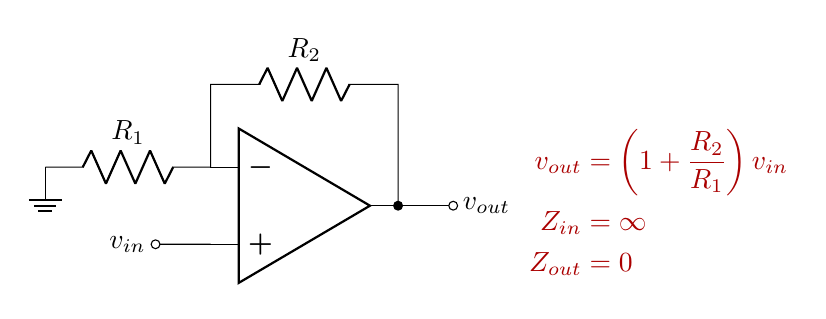
\begin{tikzpicture}
    \begin{scope}[scale=0.7]
        \draw (0, 0) node[op amp] (OpAmp) {};
        \path let \p2 = (OpAmp.out) in
            \pgfextra{
                \xdef\xout{\x2}
                \xdef\yout{\y2}
            };
        \path let \p1 = (OpAmp.-) in
            \pgfextra{
                \xdef\xin{\x1}
                \xdef\yin{\y1}
            };
        \draw (OpAmp.-)
            to[R, l_={$R_1$}] ++(-3, 0)
            node[ground] {};
        \draw (OpAmp.-)
            to[short] ++(0, 1.5)
            to[R, l={$R_2$}] ++(\xout - \xin, 0)
            to[short, -*] (OpAmp.out);
        \draw (OpAmp.out)
            to[short, -o] ++(1.0, 0)
            node[anchor=west] {$v_{out}$};
        \draw (OpAmp.+)
            to[short, -o] ++(-1.0, 0)
            node[anchor=east] {$v_{in}$};
    \end{scope}
    \begin{scope}[xshift=4.5cm, scale=0.7]
        % Title
        \node[anchor=center, color=myred] at (0, 0) {
            $\begin{aligned}
                v_{out} &= \left(1 + \frac{R_2}{R_1}\right) v_{in} \\
                Z_{in} &= \infty \\
                Z_{out} &= 0
            \end{aligned}$
        };
    \end{scope}
\end{tikzpicture}
\end{document}